\documentclass{article}
\usepackage{graphicx} % For including diagrams

\title{TCP File Transfer Practical Work 1}
\author{Ha Tan Minh}
\date{}

\begin{document}

\maketitle

\section{Introduction}
The purpose of this practical is to implement a simple file transfer system using TCP/IP. The work involves socket programming in Python, with one laptop acting as a server and the other as a client.

\section{Protocol Design}
The file transfer protocol involves:
\begin{itemize}
    \item Establishing a connection between the client and the server.
    \item Sending the file name from the client to the server.
    \item Transferring the file in chunks of data.
    \item The server saving the file after all data is received.
\end{itemize}
\begin{figure}
    \centering
    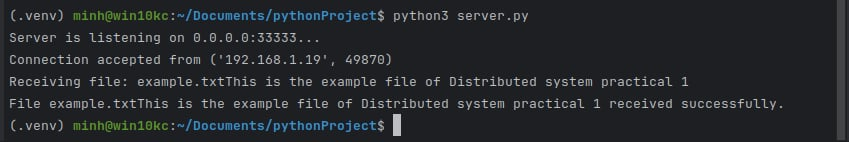
\includegraphics[width=1\linewidth]{a.png}
    \caption{Enter Caption}
    \label{fig:enter-label}
\end{figure}
\section{System Interaction}


\begin{center}
Laptop 1 (Server)
\end{center}

\begin{figure}
    \centering
    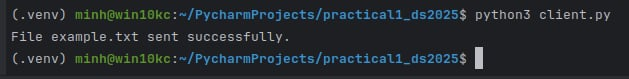
\includegraphics[width=1\linewidth]{b.png}
    \caption{Enter Caption}
    \label{fig:enter-label}
\end{figure}

\begin{center}
Laptop 2 (Client)
\end{center}
                                
\section{Implementation}
The implementation involves two Python scripts:
\subsection{Server Code}
The server listens for incoming connections and saves the file:
\begin{verbatim}
import socket

def start_server():
    server_ip = '0.0.0.0'  # Listen on all available interfaces
    server_port = 33333    # Port to listen on

    # Create a socket object
    server_socket = socket.socket(socket.AF_INET, socket.SOCK_STREAM)
    server_socket.bind((server_ip, server_port))  # Bind to the specified IP and port
    server_socket.listen(1)  # Allow one client connection at a time
    print(f"Server is listening on {server_ip}:{server_port}...")

    # Accept a connection from the client
    conn, addr = server_socket.accept()
    print(f"Connection accepted from {addr}")

    # Receive the filename from the client
    filename = conn.recv(1024).decode()
    print(f"Receiving file: {filename}")

    # Receive the file content and save it
    with open(filename, 'wb') as file:
        while True:
            data = conn.recv(1024)  # Receive data in chunks
            if not data:
                break
            file.write(data)

    print(f"File {filename} received successfully.")
    conn.close()  # Close the connection
    server_socket.close()  # Close the server socket

if __name__ == "__main__":
    start_server()


\end{verbatim}

\subsection{Client Code}
The client connects to the server and sends the file:
\begin{verbatim}
import socket

def send_file(server_ip, server_port, filename):
    # Create a socket object
    client_socket = socket.socket(socket.AF_INET, socket.SOCK_STREAM)
    client_socket.connect((server_ip, server_port))  # Connect to the server

    # Send the filename to the server
    client_socket.send(filename.encode())

    # Send the file content
    with open(filename, 'rb') as file:
        while (data := file.read(1024)):  # Read the file in chunks
            client_socket.send(data)

    print(f"File {filename} sent successfully.")
    client_socket.close()  # Close the client socket

if __name__ == "__main__":
    # Replace with the actual file name in the same directory
    server_ip = '192.168.1.20'  # Server's IP address
    server_port = 33333           # Server's port
    filename = 'example.txt'      # File to send

    send_file(server_ip, server_port, filename)


\end{verbatim}

\section{Results}
The file transfer system was successfully tested. The following results were obtained:
\begin{itemize}
    \item File transferred: `example.txt`
    \item File size: 58 B
    \item Transfer time: ~1 second
\end{itemize}

\section{Roles}
Contributed to this project:
\begin{itemize}
    \item Ha Tan Minh: Developed the server script (laptop 1).
    \item Ha Tan Minh: Developed the client script (laptop 2).
    \item Ha Tan Minh: Prepared the report in LaTeX.
\end{itemize}

\end{document}
